\documentclass{ctexart}
\usepackage[T1]{fontenc}
\usepackage[a4paper,top=1.5cm,bottom=1.5cm,left=2cm,right=2cm,marginparwidth=1.75cm]{geometry}
\usepackage{mathtools}
\usepackage{booktabs}
\usepackage{caption}
\usepackage{outlines}
\usepackage[colorlinks=false, allcolors=blue]{hyperref}
\usepackage{array}
\usepackage{makecell}
\usepackage{graphicx}
\newcolumntype{x}[1]{>{\centering\arraybackslash\hspace{0pt}}p{#1}}
\renewcommand{\tableautorefname}{表}
\DeclarePairedDelimiter{\set}{\{}{\}}
\DeclarePairedDelimiter{\paren}{(}{)}
\graphicspath{ {./images/} }
\newcommand\mc[1]{\multicolumn{1}{c}{#1}} % Note: no vertical bars
\renewcommand{\labelenumii}{(\arabic{enumii})}

\title{计算机体系结构第三次作业}
\author{卢雨轩 19071125}
% \date{\today}
\ctexset{
    section = {
        titleformat = \raggedright,
        name = {,},
        number = \chinese{section}、
    },
    paragraph = {
        runin = false
    },
    today = small,
    figurename = 图,
    contentsname = 目录,
    tablename = 表,
}

\begin{document}

\maketitle

\begin{outline}[enumerate]
    \1[3-14] 假设在一个采用组相联映像方式的cache中,主存由$B_0$~$B_7$共8块组成,cache
    有2组,每组2块,每块的大小为16B,采用LFU块替换算法。在一个程序执行过程中一次访问这个cache
    的块地址流如下:
    \begin{center}
        6,2,4,1,4,6,3,0,4,5,7,3
    \end{center}
    \2 写出主存地址的格式,并标出各字段的长度。
    \begin{center}
        \begin{tabular}{|x{3cm}|x{3cm}|x{3cm}|x{3cm}|}
            \hline
            区号1bit & 组号1bit & 块号 1bit & 块内地址 4bit \\
            \hline
        \end{tabular}
    \end{center}
    \2 写出cache地址的格式,并标出各字段的长度。
    \begin{center}
        \begin{tabular}{|x{3cm}|x{3cm}|x{3cm}|}
            \hline
            组号1bit & 块号 1bit & 块内地址 4bit \\
            \hline
        \end{tabular}
    \end{center}
    \2 画出主存与cache之间各个块的映像对应关系。
    \begin{center}
        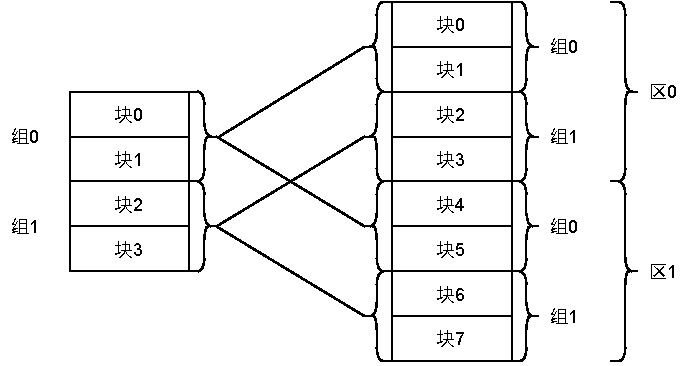
\includegraphics{homework 3 cache.drawio.pdf}
    \end{center}
    \2 如果cache的各个块号为$C_0$、$C_1$、$C_2$和$C_3$,列出程序执行
    过程中Cache的块地址流情况。
    \begin{center}
        \begin{tabular}{c|c|c|c|c|c|c|c|c|c|c|c|c|}
            \mc{主存块地址执行顺序} & \mc{6} & \mc{2} & \mc{4} & \mc{1} & \mc{4} & \mc{6} & \mc{3} & \mc{0} & \mc{4} & \mc{5} & \mc{7} & \mc{3} \\
            \cline{2-13}
            $C_0$ &   &   & 4* & 4 & 4* & 4 & 4 & 4 & 4* & 4  & 4 &4\\
            \cline{2-13}
            $C_1$ &   &   &   & 1* & 1 & 1 & 1 & 0* & 0 & 5* & 5 &5\\
            \cline{2-13}
            $C_2$ & 6* & 6 & 6 & 6 & 6  & 6* & 6 & 6 & 6 & 6 & 7* & 7\\
            \cline{2-13}
            $C_3$ &   & 2* & 2 & 2 & 2 & 2 & 3* & 3 & 3 & 3 & 3 & 3*\\
            \cline{2-13}
            \mc{操作} & \mc{\makecell{装\\入}} & \mc{\makecell{装\\入}} & \mc{\makecell{装\\入}} & \mc{\makecell{装\\入}}
             & \mc{\makecell{命\\中}} & \mc{\makecell{命\\中}} & \mc{\makecell{替\\换}} & \mc{\makecell{替\\换}} & 
             \mc{\makecell{命\\中}} & \mc{\makecell{替\\换}}  & \mc{\makecell{替\\换}} & \mc{\makecell{命\\中}}\\
        \end{tabular}
    \end{center}
    \2 如果采用FIFO替换算法,计算cache的块命中率。
    \begin{center}
        \begin{tabular}{c|c|c|c|c|c|c|c|c|c|c|c|c|}
            \mc{主存块地址执行顺序} & \mc{6} & \mc{2} & \mc{4} & \mc{1} & \mc{4} & \mc{6} & \mc{3} & \mc{0} & \mc{4} & \mc{5} & \mc{7} & \mc{3} \\
            \cline{2-13}
            $C_0$ &    &    & 4* & 4  & 4* & 4  & 4  & 0* & 0 & 5* & 5  &5\\
            \cline{2-13}
            $C_1$ &    &    &    & 1* & 1  & 1  & 1  & 1  & 4*  & 4  & 4  &4\\
            \cline{2-13}
            $C_2$ & 6* & 6  & 6  & 6  & 6  & 6* & 3* & 3  & 3  & 3  & 3 & 3*\\
            \cline{2-13}
            $C_3$ &    & 2* & 2  & 2  & 2  & 2  & 2  & 2  & 2  & 2  & 7*  & 7\\
            \cline{2-13}
            \mc{操作} & \mc{\makecell{装\\入}} & \mc{\makecell{装\\入}} & \mc{\makecell{装\\入}} & \mc{\makecell{装\\入}}
             & \mc{\makecell{命\\中}} & \mc{\makecell{命\\中}} & \mc{\makecell{替\\换}} & \mc{\makecell{替\\换}} & 
             \mc{\makecell{替\\换}} & \mc{\makecell{替\\换}}  & \mc{\makecell{替\\换}} & \mc{\makecell{命\\中}}\\
        \end{tabular}
    \end{center}
    命中率$=\frac{3}{12} = 0.25$
    \2 采用LFU替换算法,计算cache的块命中率。
    命中率$=\frac{4}{12} = 0.33$
    \1[3-16] 假设机器的时钟周期为10毫微秒,cache失效的访存时间为20个时钟周期。回答以下问题:
    \2 假设失效率为0.05,忽略写操作时的其他延迟,求机器的平均访存时间。

        $T_0 = 0.95 \times 1 + 0.05 \times 20 = 1.95\text{(cycles)} = 19.5 \text{ns}$
    \2 假设通过增加cache容量使失效率降低到0.03,但使得cache命中时的访问时间增加到了1.2时钟周期,
    指出这样的改动设计是否合适?
    
        $T_1 = 0.97 \times 1.2 + 0.03 \times 20 \approx 1.76\text{(cycles)} = 17.6 \text{ns}$\\
        可以缩短平均访问时间,改动合适。
    \2 如果时钟周期取决于cache访问时间(也就是采用延长时钟周期的方法),上述改动设计是否合适?

        不合适,会让计算密集任务显著减慢。
\end{outline}

\end{document}
